% Created by tikzDevice version 0.12.3.1 on 2021-06-14 13:33:24
% !TEX encoding = UTF-8 Unicode
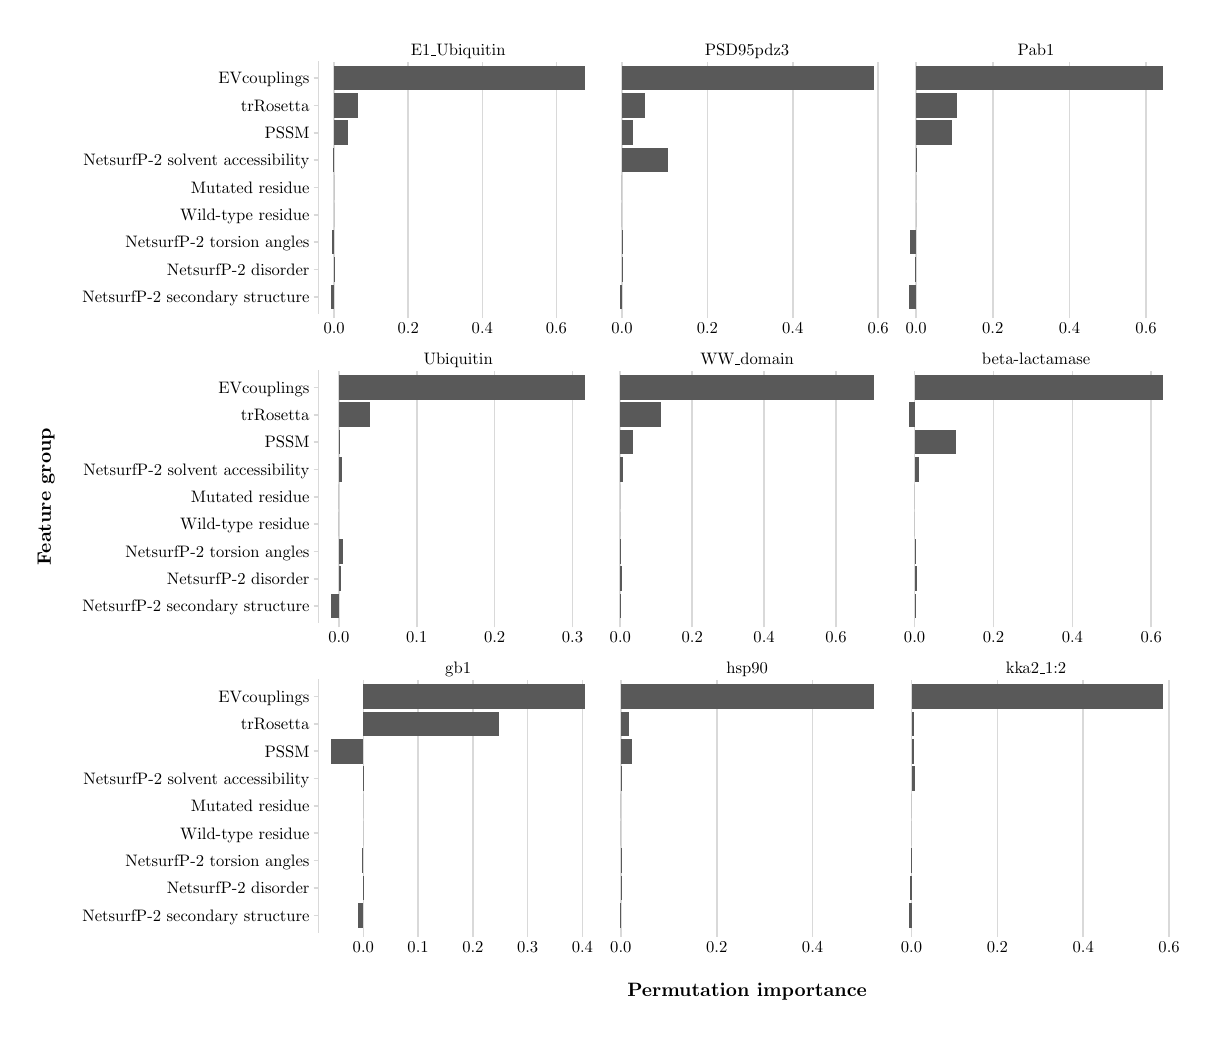
\begin{tikzpicture}[x=1pt,y=1pt]
\definecolor{fillColor}{RGB}{255,255,255}
\path[use as bounding box,fill=fillColor,fill opacity=0.00] (0,0) rectangle (418.34,354.99);
\begin{scope}
\path[clip] (105.09,251.79) rectangle (206.00,342.69);
\definecolor{drawColor}{gray}{0.85}

\path[draw=drawColor,line width= 0.6pt,line join=round] (110.76,251.79) --
	(110.76,342.69);

\path[draw=drawColor,line width= 0.6pt,line join=round] (137.53,251.79) --
	(137.53,342.69);

\path[draw=drawColor,line width= 0.6pt,line join=round] (164.29,251.79) --
	(164.29,342.69);

\path[draw=drawColor,line width= 0.6pt,line join=round] (191.06,251.79) --
	(191.06,342.69);
\definecolor{fillColor}{gray}{0.35}

\path[fill=fillColor] (110.76,322.43) rectangle (119.30,331.33);

\path[fill=fillColor] (110.76,312.55) rectangle (115.86,321.45);

\path[fill=fillColor] (110.49,302.67) rectangle (110.76,311.57);

\path[fill=fillColor] (109.68,253.27) rectangle (110.76,262.17);

\path[fill=fillColor] (110.71,263.15) rectangle (110.76,272.05);

\path[fill=fillColor] (109.89,273.03) rectangle (110.76,281.93);

\path[fill=fillColor] (110.76,332.31) rectangle (201.42,341.21);

\path[fill=fillColor] (110.76,282.91) rectangle (110.76,291.81);

\path[fill=fillColor] (110.76,292.79) rectangle (110.76,301.69);
\end{scope}
\begin{scope}
\path[clip] (105.09,140.05) rectangle (206.00,230.94);
\definecolor{drawColor}{gray}{0.85}

\path[draw=drawColor,line width= 0.6pt,line join=round] (112.45,140.05) --
	(112.45,230.94);

\path[draw=drawColor,line width= 0.6pt,line join=round] (140.59,140.05) --
	(140.59,230.94);

\path[draw=drawColor,line width= 0.6pt,line join=round] (168.73,140.05) --
	(168.73,230.94);

\path[draw=drawColor,line width= 0.6pt,line join=round] (196.87,140.05) --
	(196.87,230.94);
\definecolor{fillColor}{gray}{0.35}

\path[fill=fillColor] (112.45,210.69) rectangle (123.87,219.58);

\path[fill=fillColor] (112.45,200.81) rectangle (112.47,209.70);

\path[fill=fillColor] (112.45,190.93) rectangle (113.60,199.82);

\path[fill=fillColor] (109.68,141.53) rectangle (112.45,150.42);

\path[fill=fillColor] (112.45,151.41) rectangle (113.38,160.30);

\path[fill=fillColor] (112.45,161.29) rectangle (113.88,170.18);

\path[fill=fillColor] (112.45,220.57) rectangle (201.42,229.46);

\path[fill=fillColor] (112.45,171.17) rectangle (112.45,180.06);

\path[fill=fillColor] (112.45,181.05) rectangle (112.45,189.94);
\end{scope}
\begin{scope}
\path[clip] (105.09, 28.30) rectangle (206.00,119.20);
\definecolor{drawColor}{gray}{0.85}

\path[draw=drawColor,line width= 0.6pt,line join=round] (121.29, 28.30) --
	(121.29,119.20);

\path[draw=drawColor,line width= 0.6pt,line join=round] (141.08, 28.30) --
	(141.08,119.20);

\path[draw=drawColor,line width= 0.6pt,line join=round] (160.87, 28.30) --
	(160.87,119.20);

\path[draw=drawColor,line width= 0.6pt,line join=round] (180.66, 28.30) --
	(180.66,119.20);

\path[draw=drawColor,line width= 0.6pt,line join=round] (200.45, 28.30) --
	(200.45,119.20);
\definecolor{fillColor}{gray}{0.35}

\path[fill=fillColor] (121.29, 98.95) rectangle (170.19,107.84);

\path[fill=fillColor] (109.68, 89.07) rectangle (121.29, 97.96);

\path[fill=fillColor] (121.29, 79.19) rectangle (121.69, 88.08);

\path[fill=fillColor] (119.54, 29.79) rectangle (121.29, 38.68);

\path[fill=fillColor] (121.19, 39.67) rectangle (121.29, 48.56);

\path[fill=fillColor] (120.83, 49.55) rectangle (121.29, 58.44);

\path[fill=fillColor] (121.29,108.82) rectangle (201.42,117.72);

\path[fill=fillColor] (121.29, 59.43) rectangle (121.29, 68.32);

\path[fill=fillColor] (121.29, 69.31) rectangle (121.29, 78.20);
\end{scope}
\begin{scope}
\path[clip] (209.50,251.79) rectangle (310.42,342.69);
\definecolor{drawColor}{gray}{0.85}

\path[draw=drawColor,line width= 0.6pt,line join=round] (214.75,251.79) --
	(214.75,342.69);

\path[draw=drawColor,line width= 0.6pt,line join=round] (245.61,251.79) --
	(245.61,342.69);

\path[draw=drawColor,line width= 0.6pt,line join=round] (276.47,251.79) --
	(276.47,342.69);

\path[draw=drawColor,line width= 0.6pt,line join=round] (307.33,251.79) --
	(307.33,342.69);
\definecolor{fillColor}{gray}{0.35}

\path[fill=fillColor] (214.75,322.43) rectangle (223.22,331.33);

\path[fill=fillColor] (214.75,312.55) rectangle (218.91,321.45);

\path[fill=fillColor] (214.75,302.67) rectangle (231.39,311.57);

\path[fill=fillColor] (214.09,253.27) rectangle (214.75,262.17);

\path[fill=fillColor] (214.66,263.15) rectangle (214.75,272.05);

\path[fill=fillColor] (214.73,273.03) rectangle (214.75,281.93);

\path[fill=fillColor] (214.75,332.31) rectangle (305.83,341.21);

\path[fill=fillColor] (214.75,282.91) rectangle (214.75,291.81);

\path[fill=fillColor] (214.75,292.79) rectangle (214.75,301.69);
\end{scope}
\begin{scope}
\path[clip] (209.50,140.05) rectangle (310.42,230.94);
\definecolor{drawColor}{gray}{0.85}

\path[draw=drawColor,line width= 0.6pt,line join=round] (214.15,140.05) --
	(214.15,230.94);

\path[draw=drawColor,line width= 0.6pt,line join=round] (240.13,140.05) --
	(240.13,230.94);

\path[draw=drawColor,line width= 0.6pt,line join=round] (266.11,140.05) --
	(266.11,230.94);

\path[draw=drawColor,line width= 0.6pt,line join=round] (292.08,140.05) --
	(292.08,230.94);
\definecolor{fillColor}{gray}{0.35}

\path[fill=fillColor] (214.15,210.69) rectangle (228.78,219.58);

\path[fill=fillColor] (214.15,200.81) rectangle (218.80,209.70);

\path[fill=fillColor] (214.15,190.93) rectangle (214.96,199.82);

\path[fill=fillColor] (214.09,141.53) rectangle (214.15,150.42);

\path[fill=fillColor] (214.15,151.41) rectangle (214.78,160.30);

\path[fill=fillColor] (214.15,161.29) rectangle (214.33,170.18);

\path[fill=fillColor] (214.15,220.57) rectangle (305.83,229.46);

\path[fill=fillColor] (214.15,171.17) rectangle (214.15,180.06);

\path[fill=fillColor] (214.15,181.05) rectangle (214.15,189.94);
\end{scope}
\begin{scope}
\path[clip] (209.50, 28.30) rectangle (310.42,119.20);
\definecolor{drawColor}{gray}{0.85}

\path[draw=drawColor,line width= 0.6pt,line join=round] (214.33, 28.30) --
	(214.33,119.20);

\path[draw=drawColor,line width= 0.6pt,line join=round] (248.98, 28.30) --
	(248.98,119.20);

\path[draw=drawColor,line width= 0.6pt,line join=round] (283.63, 28.30) --
	(283.63,119.20);
\definecolor{fillColor}{gray}{0.35}

\path[fill=fillColor] (214.33, 98.95) rectangle (217.31,107.84);

\path[fill=fillColor] (214.33, 89.07) rectangle (218.52, 97.96);

\path[fill=fillColor] (214.33, 79.19) rectangle (214.34, 88.08);

\path[fill=fillColor] (214.09, 29.79) rectangle (214.33, 38.68);

\path[fill=fillColor] (214.33, 39.67) rectangle (214.57, 48.56);

\path[fill=fillColor] (214.33, 49.55) rectangle (214.52, 58.44);

\path[fill=fillColor] (214.33,108.82) rectangle (305.83,117.72);

\path[fill=fillColor] (214.33, 59.43) rectangle (214.33, 68.32);

\path[fill=fillColor] (214.33, 69.31) rectangle (214.33, 78.20);
\end{scope}
\begin{scope}
\path[clip] (313.92,251.79) rectangle (414.84,342.69);
\definecolor{drawColor}{gray}{0.85}

\path[draw=drawColor,line width= 0.6pt,line join=round] (321.05,251.79) --
	(321.05,342.69);

\path[draw=drawColor,line width= 0.6pt,line join=round] (348.75,251.79) --
	(348.75,342.69);

\path[draw=drawColor,line width= 0.6pt,line join=round] (376.45,251.79) --
	(376.45,342.69);

\path[draw=drawColor,line width= 0.6pt,line join=round] (404.14,251.79) --
	(404.14,342.69);
\definecolor{fillColor}{gray}{0.35}

\path[fill=fillColor] (321.05,322.43) rectangle (335.82,331.33);

\path[fill=fillColor] (321.05,312.55) rectangle (334.08,321.45);

\path[fill=fillColor] (321.00,302.67) rectangle (321.05,311.57);

\path[fill=fillColor] (318.51,253.27) rectangle (321.05,262.17);

\path[fill=fillColor] (320.68,263.15) rectangle (321.05,272.05);

\path[fill=fillColor] (318.83,273.03) rectangle (321.05,281.93);

\path[fill=fillColor] (321.05,332.31) rectangle (410.25,341.21);

\path[fill=fillColor] (321.05,282.91) rectangle (321.05,291.81);

\path[fill=fillColor] (321.05,292.79) rectangle (321.05,301.69);
\end{scope}
\begin{scope}
\path[clip] (313.92,140.05) rectangle (414.84,230.94);
\definecolor{drawColor}{gray}{0.85}

\path[draw=drawColor,line width= 0.6pt,line join=round] (320.49,140.05) --
	(320.49,230.94);

\path[draw=drawColor,line width= 0.6pt,line join=round] (348.99,140.05) --
	(348.99,230.94);

\path[draw=drawColor,line width= 0.6pt,line join=round] (377.50,140.05) --
	(377.50,230.94);

\path[draw=drawColor,line width= 0.6pt,line join=round] (406.00,140.05) --
	(406.00,230.94);
\definecolor{fillColor}{gray}{0.35}

\path[fill=fillColor] (318.51,210.69) rectangle (320.49,219.58);

\path[fill=fillColor] (320.49,200.81) rectangle (335.44,209.70);

\path[fill=fillColor] (320.49,190.93) rectangle (322.04,199.82);

\path[fill=fillColor] (320.49,141.53) rectangle (320.81,150.42);

\path[fill=fillColor] (320.49,151.41) rectangle (321.27,160.30);

\path[fill=fillColor] (320.49,161.29) rectangle (320.51,170.18);

\path[fill=fillColor] (320.49,220.57) rectangle (410.25,229.46);

\path[fill=fillColor] (320.49,171.17) rectangle (320.49,180.06);

\path[fill=fillColor] (320.49,181.05) rectangle (320.49,189.94);
\end{scope}
\begin{scope}
\path[clip] (313.92, 28.30) rectangle (414.84,119.20);
\definecolor{drawColor}{gray}{0.85}

\path[draw=drawColor,line width= 0.6pt,line join=round] (319.39, 28.30) --
	(319.39,119.20);

\path[draw=drawColor,line width= 0.6pt,line join=round] (350.41, 28.30) --
	(350.41,119.20);

\path[draw=drawColor,line width= 0.6pt,line join=round] (381.43, 28.30) --
	(381.43,119.20);

\path[draw=drawColor,line width= 0.6pt,line join=round] (412.45, 28.30) --
	(412.45,119.20);
\definecolor{fillColor}{gray}{0.35}

\path[fill=fillColor] (319.39, 98.95) rectangle (320.22,107.84);

\path[fill=fillColor] (319.39, 89.07) rectangle (320.27, 97.96);

\path[fill=fillColor] (319.39, 79.19) rectangle (320.60, 88.08);

\path[fill=fillColor] (318.51, 29.79) rectangle (319.39, 38.68);

\path[fill=fillColor] (318.92, 39.67) rectangle (319.39, 48.56);

\path[fill=fillColor] (319.32, 49.55) rectangle (319.39, 58.44);

\path[fill=fillColor] (319.39,108.82) rectangle (410.25,117.72);

\path[fill=fillColor] (319.39, 59.43) rectangle (319.39, 68.32);

\path[fill=fillColor] (319.39, 69.31) rectangle (319.39, 78.20);
\end{scope}
\begin{scope}
\path[clip] (105.09,119.20) rectangle (206.00,128.00);
\definecolor{drawColor}{RGB}{0,0,0}

\node[text=drawColor,anchor=base,inner sep=0pt, outer sep=0pt, scale=  0.60] at (155.55,121.53) {gb1};
\end{scope}
\begin{scope}
\path[clip] (209.50,119.20) rectangle (310.42,128.00);
\definecolor{drawColor}{RGB}{0,0,0}

\node[text=drawColor,anchor=base,inner sep=0pt, outer sep=0pt, scale=  0.60] at (259.96,121.53) {hsp90};
\end{scope}
\begin{scope}
\path[clip] (313.92,119.20) rectangle (414.84,128.00);
\definecolor{drawColor}{RGB}{0,0,0}

\node[text=drawColor,anchor=base,inner sep=0pt, outer sep=0pt, scale=  0.60] at (364.38,121.53) {kka2\_1:2};
\end{scope}
\begin{scope}
\path[clip] (105.09,230.94) rectangle (206.00,239.74);
\definecolor{drawColor}{RGB}{0,0,0}

\node[text=drawColor,anchor=base,inner sep=0pt, outer sep=0pt, scale=  0.60] at (155.55,233.28) {Ubiquitin};
\end{scope}
\begin{scope}
\path[clip] (209.50,230.94) rectangle (310.42,239.74);
\definecolor{drawColor}{RGB}{0,0,0}

\node[text=drawColor,anchor=base,inner sep=0pt, outer sep=0pt, scale=  0.60] at (259.96,233.28) {WW\_domain};
\end{scope}
\begin{scope}
\path[clip] (313.92,230.94) rectangle (414.84,239.74);
\definecolor{drawColor}{RGB}{0,0,0}

\node[text=drawColor,anchor=base,inner sep=0pt, outer sep=0pt, scale=  0.60] at (364.38,233.28) {beta-lactamase};
\end{scope}
\begin{scope}
\path[clip] (105.09,342.69) rectangle (206.00,351.49);
\definecolor{drawColor}{RGB}{0,0,0}

\node[text=drawColor,anchor=base,inner sep=0pt, outer sep=0pt, scale=  0.60] at (155.55,345.02) {E1\_Ubiquitin};
\end{scope}
\begin{scope}
\path[clip] (209.50,342.69) rectangle (310.42,351.49);
\definecolor{drawColor}{RGB}{0,0,0}

\node[text=drawColor,anchor=base,inner sep=0pt, outer sep=0pt, scale=  0.60] at (259.96,345.02) {PSD95pdz3};
\end{scope}
\begin{scope}
\path[clip] (313.92,342.69) rectangle (414.84,351.49);
\definecolor{drawColor}{RGB}{0,0,0}

\node[text=drawColor,anchor=base,inner sep=0pt, outer sep=0pt, scale=  0.60] at (364.38,345.02) {Pab1};
\end{scope}
\begin{scope}
\path[clip] (  0.00,  0.00) rectangle (418.34,354.99);
\definecolor{drawColor}{gray}{0.85}

\path[draw=drawColor,line width= 0.6pt,line join=round] (121.29, 26.55) --
	(121.29, 28.30);

\path[draw=drawColor,line width= 0.6pt,line join=round] (141.08, 26.55) --
	(141.08, 28.30);

\path[draw=drawColor,line width= 0.6pt,line join=round] (160.87, 26.55) --
	(160.87, 28.30);

\path[draw=drawColor,line width= 0.6pt,line join=round] (180.66, 26.55) --
	(180.66, 28.30);

\path[draw=drawColor,line width= 0.6pt,line join=round] (200.45, 26.55) --
	(200.45, 28.30);
\end{scope}
\begin{scope}
\path[clip] (  0.00,  0.00) rectangle (418.34,354.99);
\definecolor{drawColor}{RGB}{0,0,0}

\node[text=drawColor,anchor=base,inner sep=0pt, outer sep=0pt, scale=  0.60] at (121.29, 20.92) {0.0};

\node[text=drawColor,anchor=base,inner sep=0pt, outer sep=0pt, scale=  0.60] at (141.08, 20.92) {0.1};

\node[text=drawColor,anchor=base,inner sep=0pt, outer sep=0pt, scale=  0.60] at (160.87, 20.92) {0.2};

\node[text=drawColor,anchor=base,inner sep=0pt, outer sep=0pt, scale=  0.60] at (180.66, 20.92) {0.3};

\node[text=drawColor,anchor=base,inner sep=0pt, outer sep=0pt, scale=  0.60] at (200.45, 20.92) {0.4};
\end{scope}
\begin{scope}
\path[clip] (  0.00,  0.00) rectangle (418.34,354.99);
\definecolor{drawColor}{gray}{0.85}

\path[draw=drawColor,line width= 0.6pt,line join=round] (214.33, 26.55) --
	(214.33, 28.30);

\path[draw=drawColor,line width= 0.6pt,line join=round] (248.98, 26.55) --
	(248.98, 28.30);

\path[draw=drawColor,line width= 0.6pt,line join=round] (283.63, 26.55) --
	(283.63, 28.30);
\end{scope}
\begin{scope}
\path[clip] (  0.00,  0.00) rectangle (418.34,354.99);
\definecolor{drawColor}{RGB}{0,0,0}

\node[text=drawColor,anchor=base,inner sep=0pt, outer sep=0pt, scale=  0.60] at (214.33, 20.92) {0.0};

\node[text=drawColor,anchor=base,inner sep=0pt, outer sep=0pt, scale=  0.60] at (248.98, 20.92) {0.2};

\node[text=drawColor,anchor=base,inner sep=0pt, outer sep=0pt, scale=  0.60] at (283.63, 20.92) {0.4};
\end{scope}
\begin{scope}
\path[clip] (  0.00,  0.00) rectangle (418.34,354.99);
\definecolor{drawColor}{gray}{0.85}

\path[draw=drawColor,line width= 0.6pt,line join=round] (319.39, 26.55) --
	(319.39, 28.30);

\path[draw=drawColor,line width= 0.6pt,line join=round] (350.41, 26.55) --
	(350.41, 28.30);

\path[draw=drawColor,line width= 0.6pt,line join=round] (381.43, 26.55) --
	(381.43, 28.30);

\path[draw=drawColor,line width= 0.6pt,line join=round] (412.45, 26.55) --
	(412.45, 28.30);
\end{scope}
\begin{scope}
\path[clip] (  0.00,  0.00) rectangle (418.34,354.99);
\definecolor{drawColor}{RGB}{0,0,0}

\node[text=drawColor,anchor=base,inner sep=0pt, outer sep=0pt, scale=  0.60] at (319.39, 20.92) {0.0};

\node[text=drawColor,anchor=base,inner sep=0pt, outer sep=0pt, scale=  0.60] at (350.41, 20.92) {0.2};

\node[text=drawColor,anchor=base,inner sep=0pt, outer sep=0pt, scale=  0.60] at (381.43, 20.92) {0.4};

\node[text=drawColor,anchor=base,inner sep=0pt, outer sep=0pt, scale=  0.60] at (412.45, 20.92) {0.6};
\end{scope}
\begin{scope}
\path[clip] (  0.00,  0.00) rectangle (418.34,354.99);
\definecolor{drawColor}{gray}{0.85}

\path[draw=drawColor,line width= 0.6pt,line join=round] (112.45,138.30) --
	(112.45,140.05);

\path[draw=drawColor,line width= 0.6pt,line join=round] (140.59,138.30) --
	(140.59,140.05);

\path[draw=drawColor,line width= 0.6pt,line join=round] (168.73,138.30) --
	(168.73,140.05);

\path[draw=drawColor,line width= 0.6pt,line join=round] (196.87,138.30) --
	(196.87,140.05);
\end{scope}
\begin{scope}
\path[clip] (  0.00,  0.00) rectangle (418.34,354.99);
\definecolor{drawColor}{RGB}{0,0,0}

\node[text=drawColor,anchor=base,inner sep=0pt, outer sep=0pt, scale=  0.60] at (112.45,132.67) {0.0};

\node[text=drawColor,anchor=base,inner sep=0pt, outer sep=0pt, scale=  0.60] at (140.59,132.67) {0.1};

\node[text=drawColor,anchor=base,inner sep=0pt, outer sep=0pt, scale=  0.60] at (168.73,132.67) {0.2};

\node[text=drawColor,anchor=base,inner sep=0pt, outer sep=0pt, scale=  0.60] at (196.87,132.67) {0.3};
\end{scope}
\begin{scope}
\path[clip] (  0.00,  0.00) rectangle (418.34,354.99);
\definecolor{drawColor}{gray}{0.85}

\path[draw=drawColor,line width= 0.6pt,line join=round] (214.15,138.30) --
	(214.15,140.05);

\path[draw=drawColor,line width= 0.6pt,line join=round] (240.13,138.30) --
	(240.13,140.05);

\path[draw=drawColor,line width= 0.6pt,line join=round] (266.11,138.30) --
	(266.11,140.05);

\path[draw=drawColor,line width= 0.6pt,line join=round] (292.08,138.30) --
	(292.08,140.05);
\end{scope}
\begin{scope}
\path[clip] (  0.00,  0.00) rectangle (418.34,354.99);
\definecolor{drawColor}{RGB}{0,0,0}

\node[text=drawColor,anchor=base,inner sep=0pt, outer sep=0pt, scale=  0.60] at (214.15,132.67) {0.0};

\node[text=drawColor,anchor=base,inner sep=0pt, outer sep=0pt, scale=  0.60] at (240.13,132.67) {0.2};

\node[text=drawColor,anchor=base,inner sep=0pt, outer sep=0pt, scale=  0.60] at (266.11,132.67) {0.4};

\node[text=drawColor,anchor=base,inner sep=0pt, outer sep=0pt, scale=  0.60] at (292.08,132.67) {0.6};
\end{scope}
\begin{scope}
\path[clip] (  0.00,  0.00) rectangle (418.34,354.99);
\definecolor{drawColor}{gray}{0.85}

\path[draw=drawColor,line width= 0.6pt,line join=round] (320.49,138.30) --
	(320.49,140.05);

\path[draw=drawColor,line width= 0.6pt,line join=round] (348.99,138.30) --
	(348.99,140.05);

\path[draw=drawColor,line width= 0.6pt,line join=round] (377.50,138.30) --
	(377.50,140.05);

\path[draw=drawColor,line width= 0.6pt,line join=round] (406.00,138.30) --
	(406.00,140.05);
\end{scope}
\begin{scope}
\path[clip] (  0.00,  0.00) rectangle (418.34,354.99);
\definecolor{drawColor}{RGB}{0,0,0}

\node[text=drawColor,anchor=base,inner sep=0pt, outer sep=0pt, scale=  0.60] at (320.49,132.67) {0.0};

\node[text=drawColor,anchor=base,inner sep=0pt, outer sep=0pt, scale=  0.60] at (348.99,132.67) {0.2};

\node[text=drawColor,anchor=base,inner sep=0pt, outer sep=0pt, scale=  0.60] at (377.50,132.67) {0.4};

\node[text=drawColor,anchor=base,inner sep=0pt, outer sep=0pt, scale=  0.60] at (406.00,132.67) {0.6};
\end{scope}
\begin{scope}
\path[clip] (  0.00,  0.00) rectangle (418.34,354.99);
\definecolor{drawColor}{gray}{0.85}

\path[draw=drawColor,line width= 0.6pt,line join=round] (110.76,250.04) --
	(110.76,251.79);

\path[draw=drawColor,line width= 0.6pt,line join=round] (137.53,250.04) --
	(137.53,251.79);

\path[draw=drawColor,line width= 0.6pt,line join=round] (164.29,250.04) --
	(164.29,251.79);

\path[draw=drawColor,line width= 0.6pt,line join=round] (191.06,250.04) --
	(191.06,251.79);
\end{scope}
\begin{scope}
\path[clip] (  0.00,  0.00) rectangle (418.34,354.99);
\definecolor{drawColor}{RGB}{0,0,0}

\node[text=drawColor,anchor=base,inner sep=0pt, outer sep=0pt, scale=  0.60] at (110.76,244.41) {0.0};

\node[text=drawColor,anchor=base,inner sep=0pt, outer sep=0pt, scale=  0.60] at (137.53,244.41) {0.2};

\node[text=drawColor,anchor=base,inner sep=0pt, outer sep=0pt, scale=  0.60] at (164.29,244.41) {0.4};

\node[text=drawColor,anchor=base,inner sep=0pt, outer sep=0pt, scale=  0.60] at (191.06,244.41) {0.6};
\end{scope}
\begin{scope}
\path[clip] (  0.00,  0.00) rectangle (418.34,354.99);
\definecolor{drawColor}{gray}{0.85}

\path[draw=drawColor,line width= 0.6pt,line join=round] (214.75,250.04) --
	(214.75,251.79);

\path[draw=drawColor,line width= 0.6pt,line join=round] (245.61,250.04) --
	(245.61,251.79);

\path[draw=drawColor,line width= 0.6pt,line join=round] (276.47,250.04) --
	(276.47,251.79);

\path[draw=drawColor,line width= 0.6pt,line join=round] (307.33,250.04) --
	(307.33,251.79);
\end{scope}
\begin{scope}
\path[clip] (  0.00,  0.00) rectangle (418.34,354.99);
\definecolor{drawColor}{RGB}{0,0,0}

\node[text=drawColor,anchor=base,inner sep=0pt, outer sep=0pt, scale=  0.60] at (214.75,244.41) {0.0};

\node[text=drawColor,anchor=base,inner sep=0pt, outer sep=0pt, scale=  0.60] at (245.61,244.41) {0.2};

\node[text=drawColor,anchor=base,inner sep=0pt, outer sep=0pt, scale=  0.60] at (276.47,244.41) {0.4};

\node[text=drawColor,anchor=base,inner sep=0pt, outer sep=0pt, scale=  0.60] at (307.33,244.41) {0.6};
\end{scope}
\begin{scope}
\path[clip] (  0.00,  0.00) rectangle (418.34,354.99);
\definecolor{drawColor}{gray}{0.85}

\path[draw=drawColor,line width= 0.6pt,line join=round] (321.05,250.04) --
	(321.05,251.79);

\path[draw=drawColor,line width= 0.6pt,line join=round] (348.75,250.04) --
	(348.75,251.79);

\path[draw=drawColor,line width= 0.6pt,line join=round] (376.45,250.04) --
	(376.45,251.79);

\path[draw=drawColor,line width= 0.6pt,line join=round] (404.14,250.04) --
	(404.14,251.79);
\end{scope}
\begin{scope}
\path[clip] (  0.00,  0.00) rectangle (418.34,354.99);
\definecolor{drawColor}{RGB}{0,0,0}

\node[text=drawColor,anchor=base,inner sep=0pt, outer sep=0pt, scale=  0.60] at (321.05,244.41) {0.0};

\node[text=drawColor,anchor=base,inner sep=0pt, outer sep=0pt, scale=  0.60] at (348.75,244.41) {0.2};

\node[text=drawColor,anchor=base,inner sep=0pt, outer sep=0pt, scale=  0.60] at (376.45,244.41) {0.4};

\node[text=drawColor,anchor=base,inner sep=0pt, outer sep=0pt, scale=  0.60] at (404.14,244.41) {0.6};
\end{scope}
\begin{scope}
\path[clip] (  0.00,  0.00) rectangle (418.34,354.99);
\definecolor{drawColor}{gray}{0.85}

\path[draw=drawColor,line width= 0.6pt,line join=round,line cap=rect] (105.09,251.79) --
	(105.09,342.69);
\end{scope}
\begin{scope}
\path[clip] (  0.00,  0.00) rectangle (418.34,354.99);
\definecolor{drawColor}{RGB}{0,0,0}

\node[text=drawColor,anchor=base east,inner sep=0pt, outer sep=0pt, scale=  0.60] at (101.84,255.65) {NetsurfP-2 secondary structure};

\node[text=drawColor,anchor=base east,inner sep=0pt, outer sep=0pt, scale=  0.60] at (101.84,265.53) {NetsurfP-2 disorder};

\node[text=drawColor,anchor=base east,inner sep=0pt, outer sep=0pt, scale=  0.60] at (101.84,275.41) {NetsurfP-2 torsion angles};

\node[text=drawColor,anchor=base east,inner sep=0pt, outer sep=0pt, scale=  0.60] at (101.84,285.29) {Wild-type residue};

\node[text=drawColor,anchor=base east,inner sep=0pt, outer sep=0pt, scale=  0.60] at (101.84,295.17) {Mutated residue};

\node[text=drawColor,anchor=base east,inner sep=0pt, outer sep=0pt, scale=  0.60] at (101.84,305.05) {NetsurfP-2 solvent accessibility};

\node[text=drawColor,anchor=base east,inner sep=0pt, outer sep=0pt, scale=  0.60] at (101.84,314.93) {PSSM};

\node[text=drawColor,anchor=base east,inner sep=0pt, outer sep=0pt, scale=  0.60] at (101.84,324.81) {trRosetta};

\node[text=drawColor,anchor=base east,inner sep=0pt, outer sep=0pt, scale=  0.60] at (101.84,334.69) {EVcouplings};
\end{scope}
\begin{scope}
\path[clip] (  0.00,  0.00) rectangle (418.34,354.99);
\definecolor{drawColor}{gray}{0.85}

\path[draw=drawColor,line width= 0.6pt,line join=round] (103.34,257.72) --
	(105.09,257.72);

\path[draw=drawColor,line width= 0.6pt,line join=round] (103.34,267.60) --
	(105.09,267.60);

\path[draw=drawColor,line width= 0.6pt,line join=round] (103.34,277.48) --
	(105.09,277.48);

\path[draw=drawColor,line width= 0.6pt,line join=round] (103.34,287.36) --
	(105.09,287.36);

\path[draw=drawColor,line width= 0.6pt,line join=round] (103.34,297.24) --
	(105.09,297.24);

\path[draw=drawColor,line width= 0.6pt,line join=round] (103.34,307.12) --
	(105.09,307.12);

\path[draw=drawColor,line width= 0.6pt,line join=round] (103.34,317.00) --
	(105.09,317.00);

\path[draw=drawColor,line width= 0.6pt,line join=round] (103.34,326.88) --
	(105.09,326.88);

\path[draw=drawColor,line width= 0.6pt,line join=round] (103.34,336.76) --
	(105.09,336.76);
\end{scope}
\begin{scope}
\path[clip] (  0.00,  0.00) rectangle (418.34,354.99);
\definecolor{drawColor}{gray}{0.85}

\path[draw=drawColor,line width= 0.6pt,line join=round,line cap=rect] (105.09,140.05) --
	(105.09,230.94);
\end{scope}
\begin{scope}
\path[clip] (  0.00,  0.00) rectangle (418.34,354.99);
\definecolor{drawColor}{RGB}{0,0,0}

\node[text=drawColor,anchor=base east,inner sep=0pt, outer sep=0pt, scale=  0.60] at (101.84,143.91) {NetsurfP-2 secondary structure};

\node[text=drawColor,anchor=base east,inner sep=0pt, outer sep=0pt, scale=  0.60] at (101.84,153.79) {NetsurfP-2 disorder};

\node[text=drawColor,anchor=base east,inner sep=0pt, outer sep=0pt, scale=  0.60] at (101.84,163.67) {NetsurfP-2 torsion angles};

\node[text=drawColor,anchor=base east,inner sep=0pt, outer sep=0pt, scale=  0.60] at (101.84,173.55) {Wild-type residue};

\node[text=drawColor,anchor=base east,inner sep=0pt, outer sep=0pt, scale=  0.60] at (101.84,183.43) {Mutated residue};

\node[text=drawColor,anchor=base east,inner sep=0pt, outer sep=0pt, scale=  0.60] at (101.84,193.31) {NetsurfP-2 solvent accessibility};

\node[text=drawColor,anchor=base east,inner sep=0pt, outer sep=0pt, scale=  0.60] at (101.84,203.19) {PSSM};

\node[text=drawColor,anchor=base east,inner sep=0pt, outer sep=0pt, scale=  0.60] at (101.84,213.07) {trRosetta};

\node[text=drawColor,anchor=base east,inner sep=0pt, outer sep=0pt, scale=  0.60] at (101.84,222.95) {EVcouplings};
\end{scope}
\begin{scope}
\path[clip] (  0.00,  0.00) rectangle (418.34,354.99);
\definecolor{drawColor}{gray}{0.85}

\path[draw=drawColor,line width= 0.6pt,line join=round] (103.34,145.98) --
	(105.09,145.98);

\path[draw=drawColor,line width= 0.6pt,line join=round] (103.34,155.86) --
	(105.09,155.86);

\path[draw=drawColor,line width= 0.6pt,line join=round] (103.34,165.74) --
	(105.09,165.74);

\path[draw=drawColor,line width= 0.6pt,line join=round] (103.34,175.62) --
	(105.09,175.62);

\path[draw=drawColor,line width= 0.6pt,line join=round] (103.34,185.50) --
	(105.09,185.50);

\path[draw=drawColor,line width= 0.6pt,line join=round] (103.34,195.38) --
	(105.09,195.38);

\path[draw=drawColor,line width= 0.6pt,line join=round] (103.34,205.26) --
	(105.09,205.26);

\path[draw=drawColor,line width= 0.6pt,line join=round] (103.34,215.14) --
	(105.09,215.14);

\path[draw=drawColor,line width= 0.6pt,line join=round] (103.34,225.02) --
	(105.09,225.02);
\end{scope}
\begin{scope}
\path[clip] (  0.00,  0.00) rectangle (418.34,354.99);
\definecolor{drawColor}{gray}{0.85}

\path[draw=drawColor,line width= 0.6pt,line join=round,line cap=rect] (105.09, 28.30) --
	(105.09,119.20);
\end{scope}
\begin{scope}
\path[clip] (  0.00,  0.00) rectangle (418.34,354.99);
\definecolor{drawColor}{RGB}{0,0,0}

\node[text=drawColor,anchor=base east,inner sep=0pt, outer sep=0pt, scale=  0.60] at (101.84, 32.17) {NetsurfP-2 secondary structure};

\node[text=drawColor,anchor=base east,inner sep=0pt, outer sep=0pt, scale=  0.60] at (101.84, 42.05) {NetsurfP-2 disorder};

\node[text=drawColor,anchor=base east,inner sep=0pt, outer sep=0pt, scale=  0.60] at (101.84, 51.93) {NetsurfP-2 torsion angles};

\node[text=drawColor,anchor=base east,inner sep=0pt, outer sep=0pt, scale=  0.60] at (101.84, 61.81) {Wild-type residue};

\node[text=drawColor,anchor=base east,inner sep=0pt, outer sep=0pt, scale=  0.60] at (101.84, 71.68) {Mutated residue};

\node[text=drawColor,anchor=base east,inner sep=0pt, outer sep=0pt, scale=  0.60] at (101.84, 81.56) {NetsurfP-2 solvent accessibility};

\node[text=drawColor,anchor=base east,inner sep=0pt, outer sep=0pt, scale=  0.60] at (101.84, 91.44) {PSSM};

\node[text=drawColor,anchor=base east,inner sep=0pt, outer sep=0pt, scale=  0.60] at (101.84,101.32) {trRosetta};

\node[text=drawColor,anchor=base east,inner sep=0pt, outer sep=0pt, scale=  0.60] at (101.84,111.20) {EVcouplings};
\end{scope}
\begin{scope}
\path[clip] (  0.00,  0.00) rectangle (418.34,354.99);
\definecolor{drawColor}{gray}{0.85}

\path[draw=drawColor,line width= 0.6pt,line join=round] (103.34, 34.23) --
	(105.09, 34.23);

\path[draw=drawColor,line width= 0.6pt,line join=round] (103.34, 44.11) --
	(105.09, 44.11);

\path[draw=drawColor,line width= 0.6pt,line join=round] (103.34, 53.99) --
	(105.09, 53.99);

\path[draw=drawColor,line width= 0.6pt,line join=round] (103.34, 63.87) --
	(105.09, 63.87);

\path[draw=drawColor,line width= 0.6pt,line join=round] (103.34, 73.75) --
	(105.09, 73.75);

\path[draw=drawColor,line width= 0.6pt,line join=round] (103.34, 83.63) --
	(105.09, 83.63);

\path[draw=drawColor,line width= 0.6pt,line join=round] (103.34, 93.51) --
	(105.09, 93.51);

\path[draw=drawColor,line width= 0.6pt,line join=round] (103.34,103.39) --
	(105.09,103.39);

\path[draw=drawColor,line width= 0.6pt,line join=round] (103.34,113.27) --
	(105.09,113.27);
\end{scope}
\begin{scope}
\path[clip] (  0.00,  0.00) rectangle (418.34,354.99);
\definecolor{drawColor}{RGB}{0,0,0}

\node[text=drawColor,anchor=base,inner sep=0pt, outer sep=0pt, scale=  0.70] at (259.96,  4.86) {\bfseries Permutation importance};
\end{scope}
\begin{scope}
\path[clip] (  0.00,  0.00) rectangle (418.34,354.99);
\definecolor{drawColor}{RGB}{0,0,0}

\node[text=drawColor,rotate= 90.00,anchor=base,inner sep=0pt, outer sep=0pt, scale=  0.70] at (  8.39,185.50) {\bfseries Feature group};
\end{scope}
\end{tikzpicture}%
